\documentclass[../main.tex]{subfiles}
\graphicspath{{\subfix{../images/}}}

\begin{document}

\begin{newrequirements}
    \begin{todolist}
    \item Actual Design description with pictures 
        and diagrams. E.g., a “wiring diagram” 
        of the implemented hardware can be 
        added. 

    \item Actual images of various modules must 
        be included wherever possible. 
        Otherwise, at least the images of 
        various aspects of the completed design 
        must be shown. 

    \item List the different tools and framework 
        used for the implementation. 

    \item Discuss any novel aspects of your 
        implementation (if applicable). You may 
        link this aspect of your design to the 
        comparison table at the end of 
        literature review and elaborate on the 
        steps taken in achieving these 
        novelties in your design. 

    \item Discuss the challenges encountered 
        during the implementation and how they 
        were addressed. 

    \item You may organize any of the above 
        recommended points as subsections 

    \end{todolist}
\end{newrequirements}

\subsection{Hardware}

The most critical parts in the hardware
architecture are the Raspberry Pi and the drone. 
We started by configuring the Raspberry Pi micro\textsc{sd} card,
flashed it with Ubuntu 18.04 desktop version,
and installed Parrot Olympe successfully. 
Then we plugged in the Wi-Fi dongle adapter
in a \textsc{usb}~2.0 port in the Raspberry Pi, 
and the \textsc{os} discovered it automatically. 

Now everything is ready to test the 
\anafi drone, so we have connected the
Raspberry Pi to the drone using built-in WiFi
to allow Raspberry to send/receive control and status 
instructions to the drone. 
For connecting Raspberry Pi and the laptop, 
we used the external WiFi adapter and turned 
on the hotspot feature to create an access point,
and this made the process so convenient because 
once the Raspberry Pi boots up, it turns on the 
access point, and the user can connect to it 
easily and execute scripts using \textsc{ssh} 
protocol or open the graphical interface 
control using the \textsc{vnc} feature.

We executed the takeoff and move forward scripts,
and it worked successfully, so we got the green 
light to continue. 
Regarding the power supply we were thinking 
of modifying the drone's battery by removing the 
plastic shield because of the drone's payload restrictions 
and limitations, but everything changed after testing 
the drone's maximum payload. As shown in \cref{fig:payload}
we attached \SI{190}{grams} of Raspberry Pi and Arduino boards
to see the effect on the performance and flight and
battery drain percentage. 
The drone has taken off  successfully, 
and the flight was normal but, we faced an expected 
battery drain that went from 
\SI{100}{\percent} to \SI{90}{\percent} in 
\SI{1.5}{minutes}.
This means the drone can fly up to 
\SI{15}{minutes} which is \SI{10}{minutes} 
less than the default battery time 
which will be considered in design constraints.
In our case, the total weight of our parts is equal
to \SI{170}{grams} which will add small time
to the battery life.

\begin{figure}[bp]
	\centering
	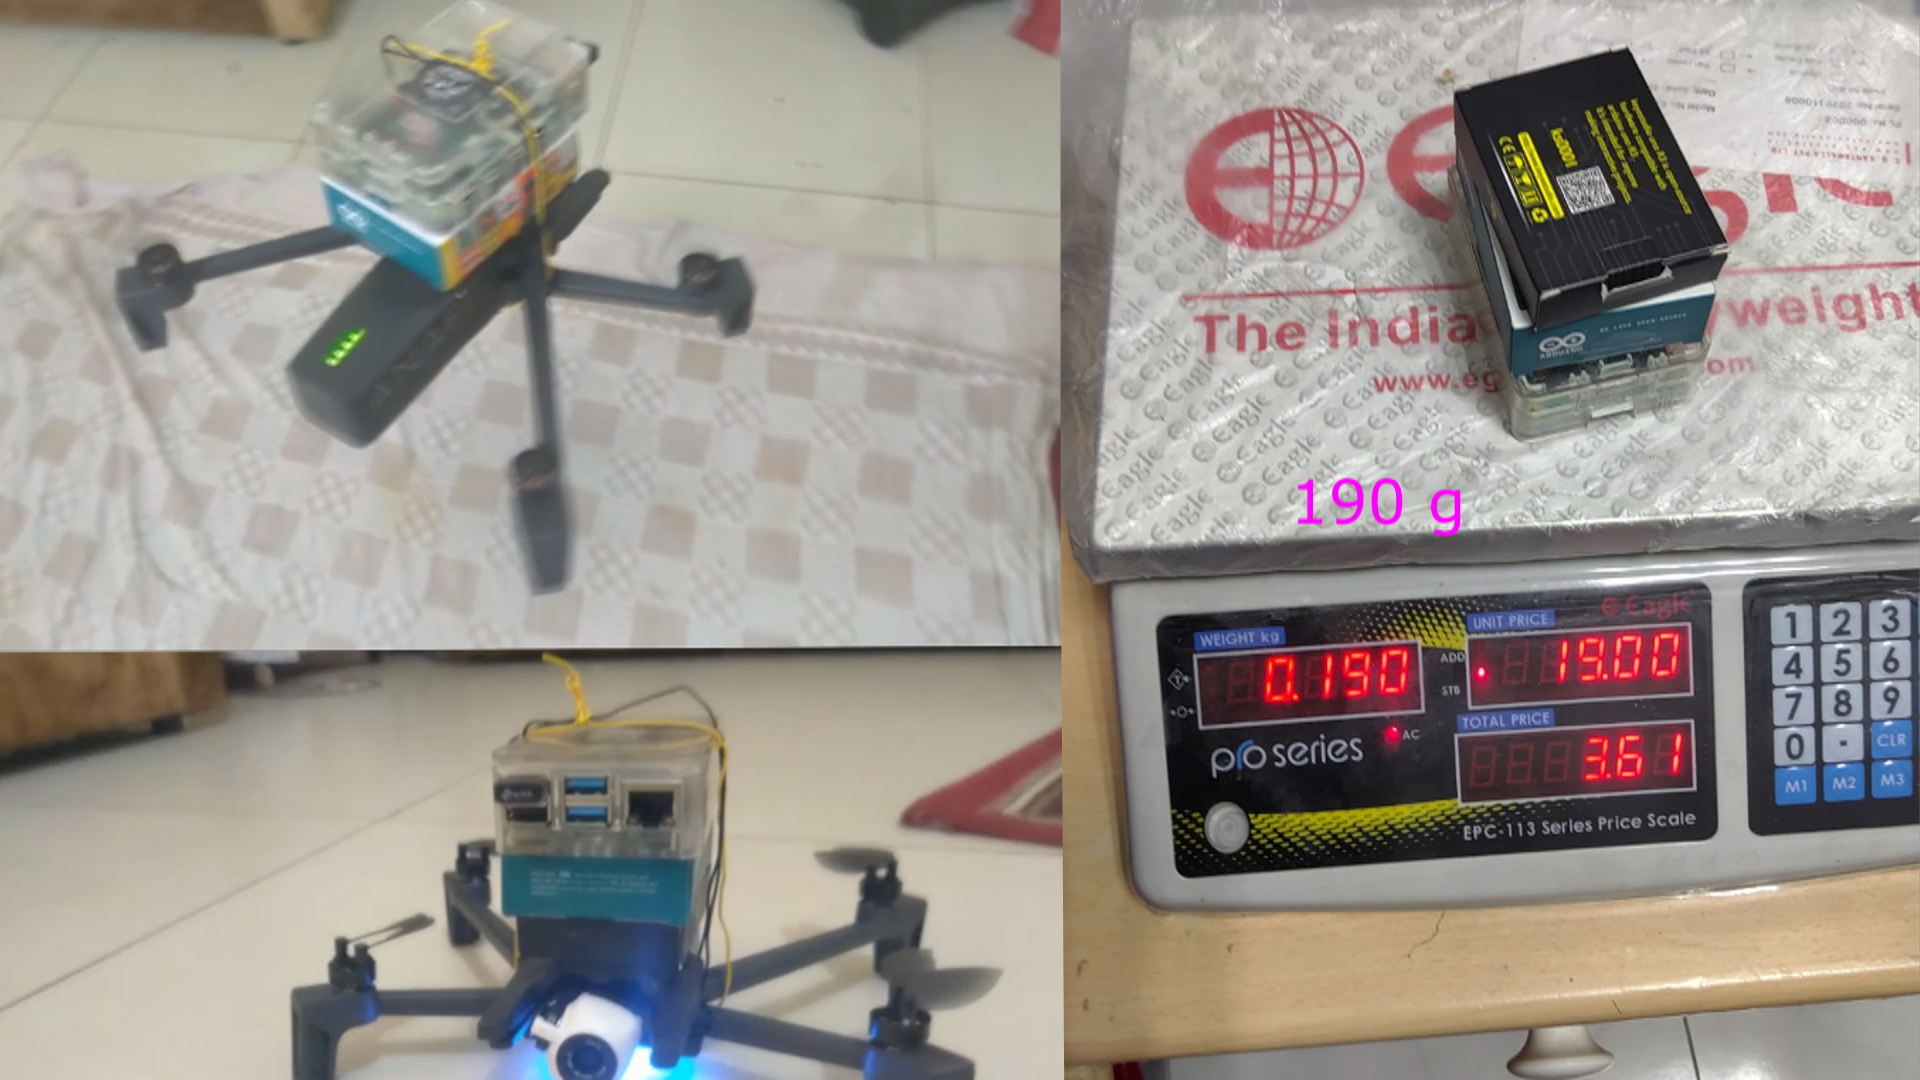
\includegraphics[width=0.6\textwidth]{payload.png}
	\caption{The payload of the drone.}
	\label{fig:payload}
\end{figure} 


We have done another experiment regarding the response time 
of the drone after sending a command to it from the Raspberry Pi. 
Calculating the response time was by starting a timer when 
sending the command and stopping it when the 
state of the drone changes. 
The experiment was done on simulation using Sphinx,
then we have moved to the real world using the \anafi drone.
From \cref{tab:respone-time}, 
we can see that all the results are less than \SI{1}{second}
which satisfied our response time constraint.
Another thing we can conclude from the table is that 
the response time of the real world is less than 
the simulation, and this is predictable since the simulation
depends on the \textsc{gpu} power and processing time. 

\begin{table}[tbp]
	\centering
	\caption{The average response time of the drone after sending a control command.}
	\label{tab:respone-time}
	\begin{tabularx}{0.7\textwidth}{ X c c }
		\toprule
		\textit{} & \textit{Simulation} & \textit{Real-world}\\ \midrule
		Motor ramping for takeoff (seconds)  & 0.3506 & 0.0323     \\
		Move while flying (seconds) & 0.7441  & 0.1511   \\
		\bottomrule
	\end{tabularx}
\end{table} 

For the Raspberry Pi power supply, we have ordered it 
online because it is not available locally, and 
it arrived after 17 days at the post office.
Regarding the connection, there are 
two different options as shown in \cref{fig:connection}.
For option A we can use \textsc{usb}-A to power the Raspberry directly without
need to solder any wires,
but there is some internal resistance.
In option B, it powers the Raspberry Pi through the \textsc{gpio} 
interface by soldering two wires to the power board and 
connecting to pin 4 and 6 in the Raspberry Pi board.
This option has small internal resistance compared to option A.
For simplicity, we will choose option A and we will 
follow the instruction of the manufacturer by choosing 
the thickest and shortest possible \textsc{usb} cable to reduce 
the power loss and voltage drops~\cite{makerfocus}.

\begin{figure}[p]
	\centering
	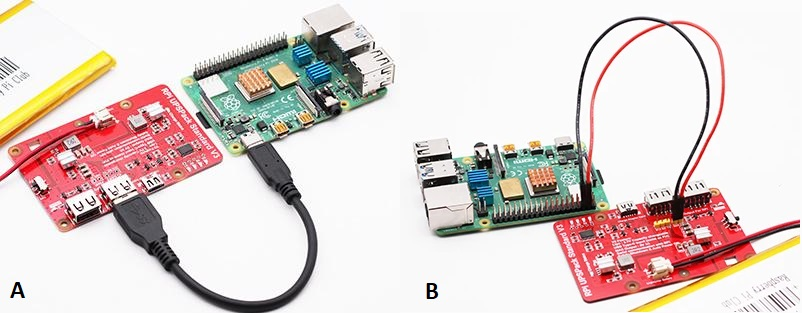
\includegraphics[width=0.5\textwidth]{connection.png}
	\caption{The Raspberry Pi and power board connection.}
	\label{fig:connection}
\end{figure}   

Since all the components are available as shown 
in \cref{fig:components}, we can now assemble 
all the parts in one piece and start testing the whole system.
We have used the zip tie to hold the components and to
make sure everything sticks together. After trying to use the 
nylon straps tape to attach the components to the drone 
we have figured out that it blocks the fan 
and sensors in the bottom of the drone, 
so normal wires attached to the sides of the drone were 
used as a temporary solution. Also, we are considering 
designing a 3D printed holder to make the process more 
flexible and convenient in future advancements, but for now,
we will stick with the simpler way. As shown in 
\cref{fig:full-hardware}, all the parts are in one system. 
The test flight was smooth, and everything works perfectly. 

\begin{figure}[p]
	\centering
	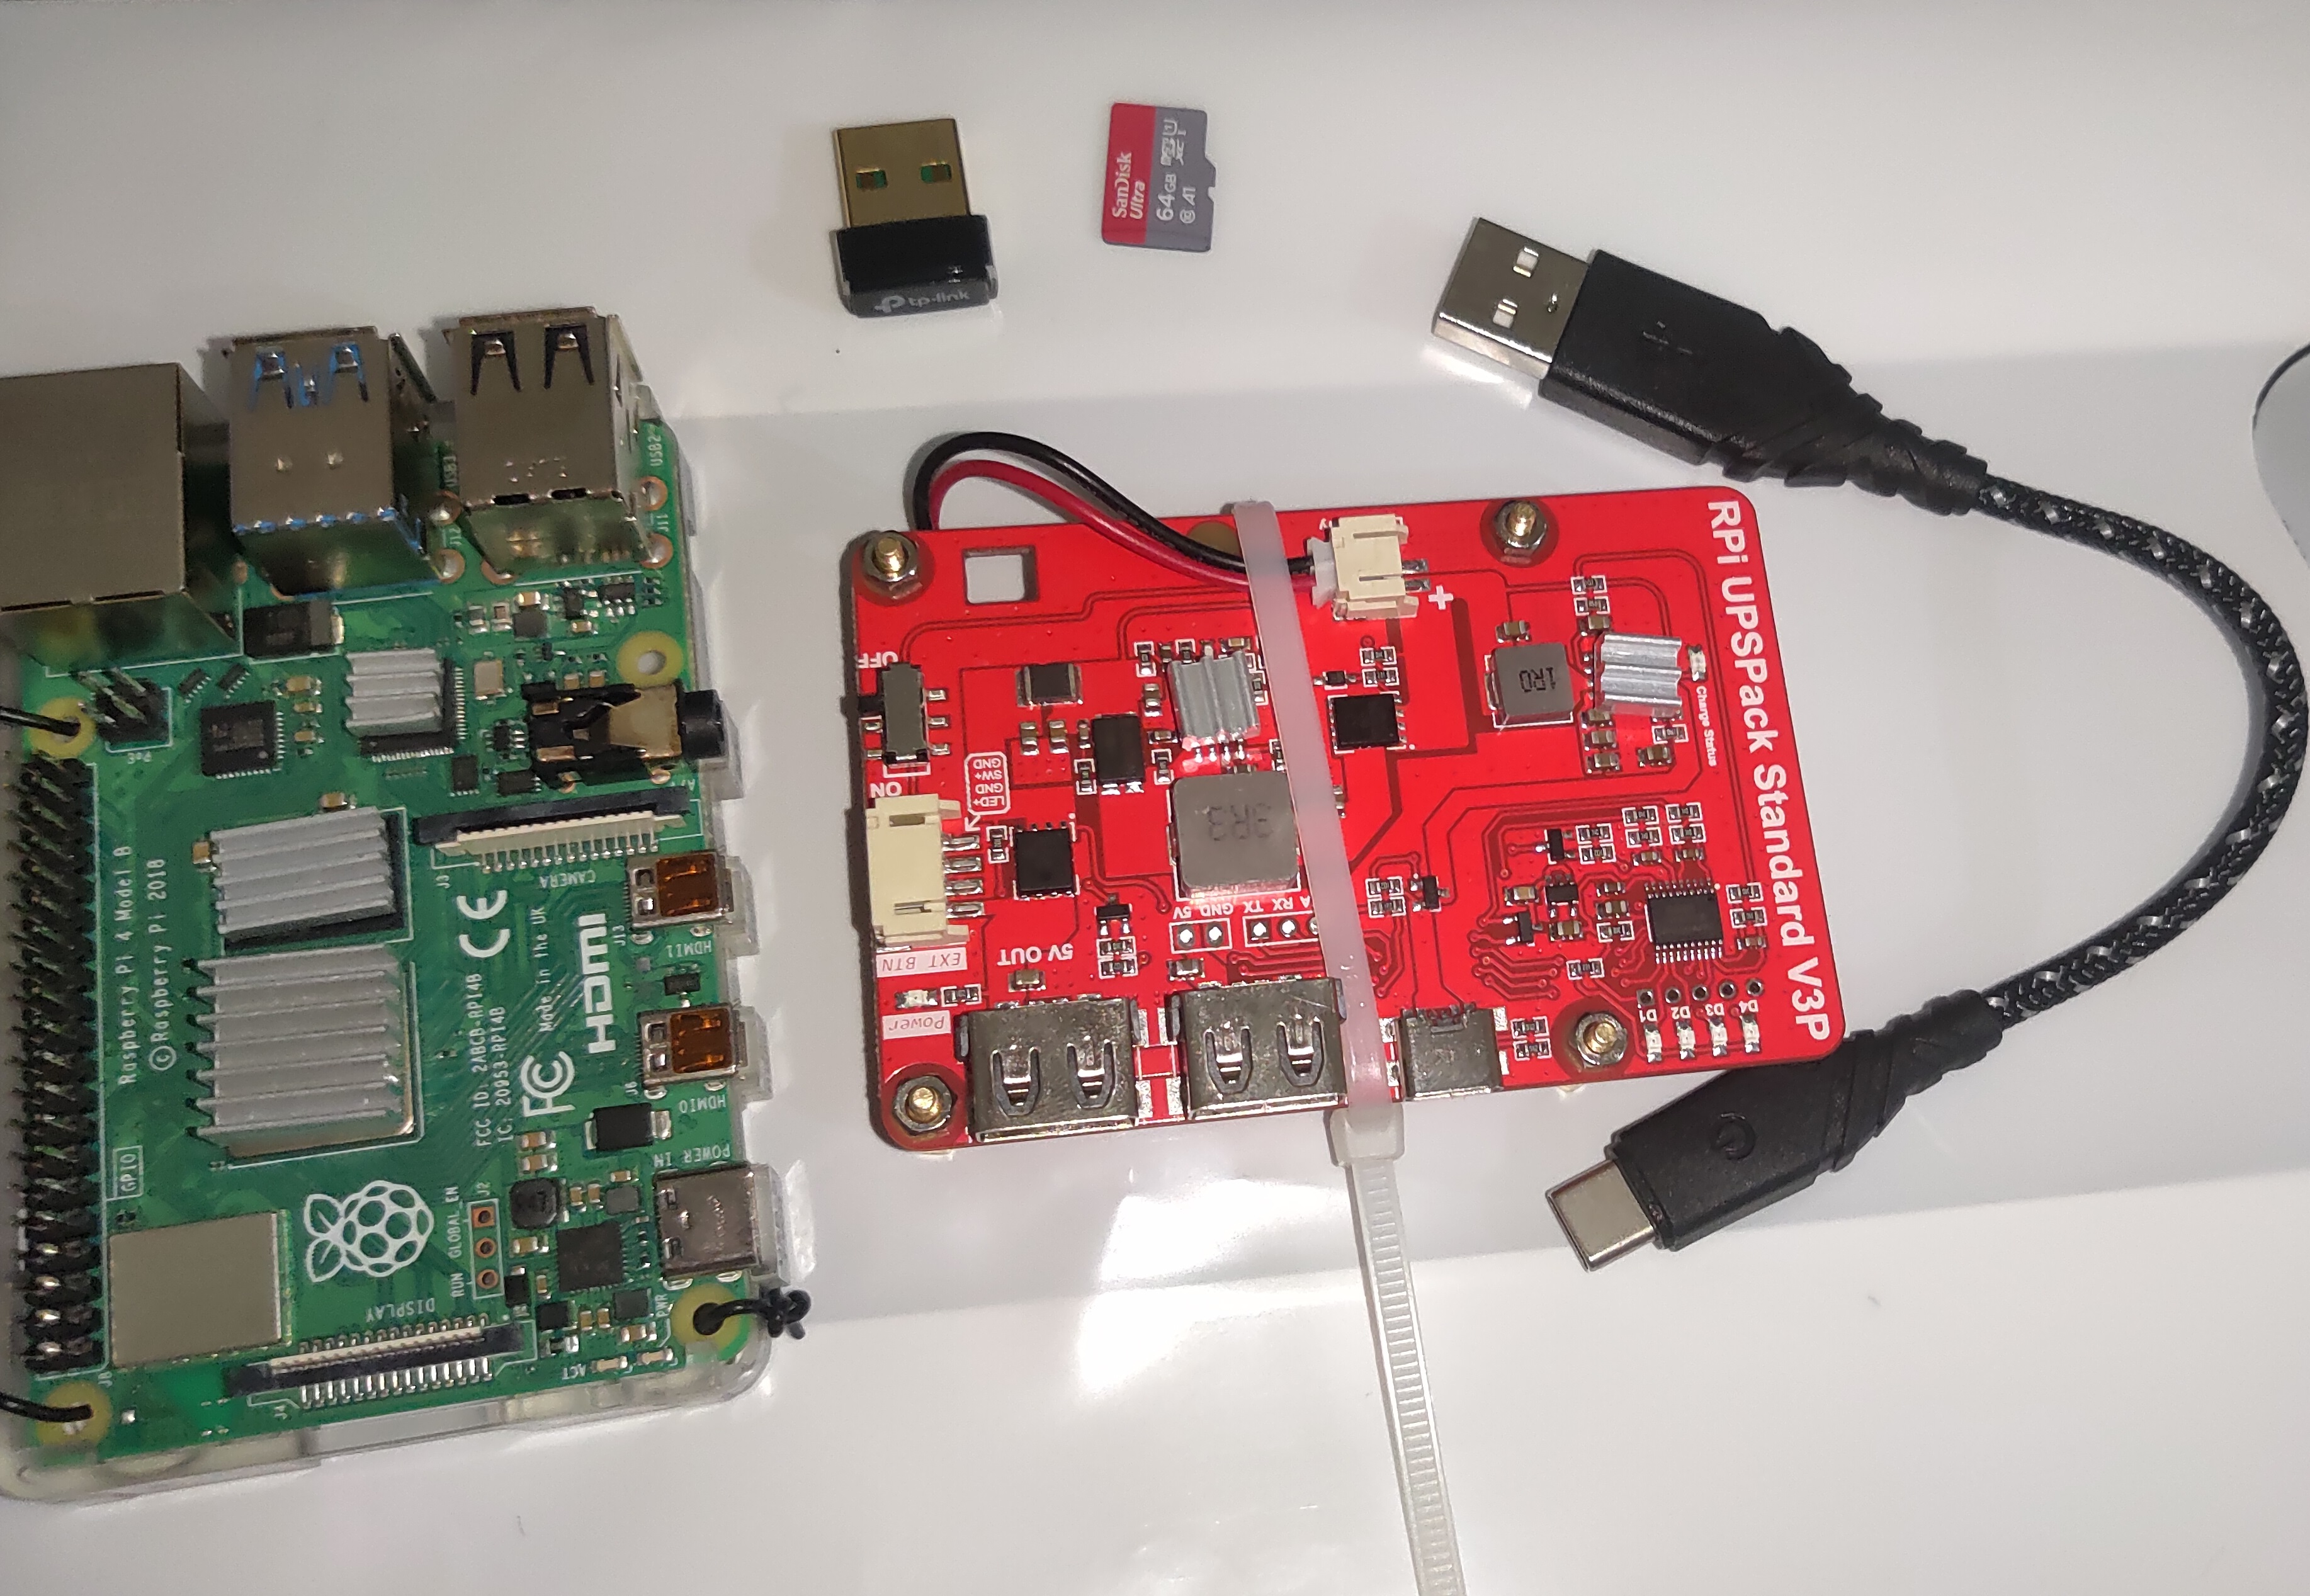
\includegraphics[width=0.5\textwidth]{components.jpg}
	\caption{All components needed.}
	\label{fig:components}
\end{figure}

\begin{figure}[p]
	\centering
	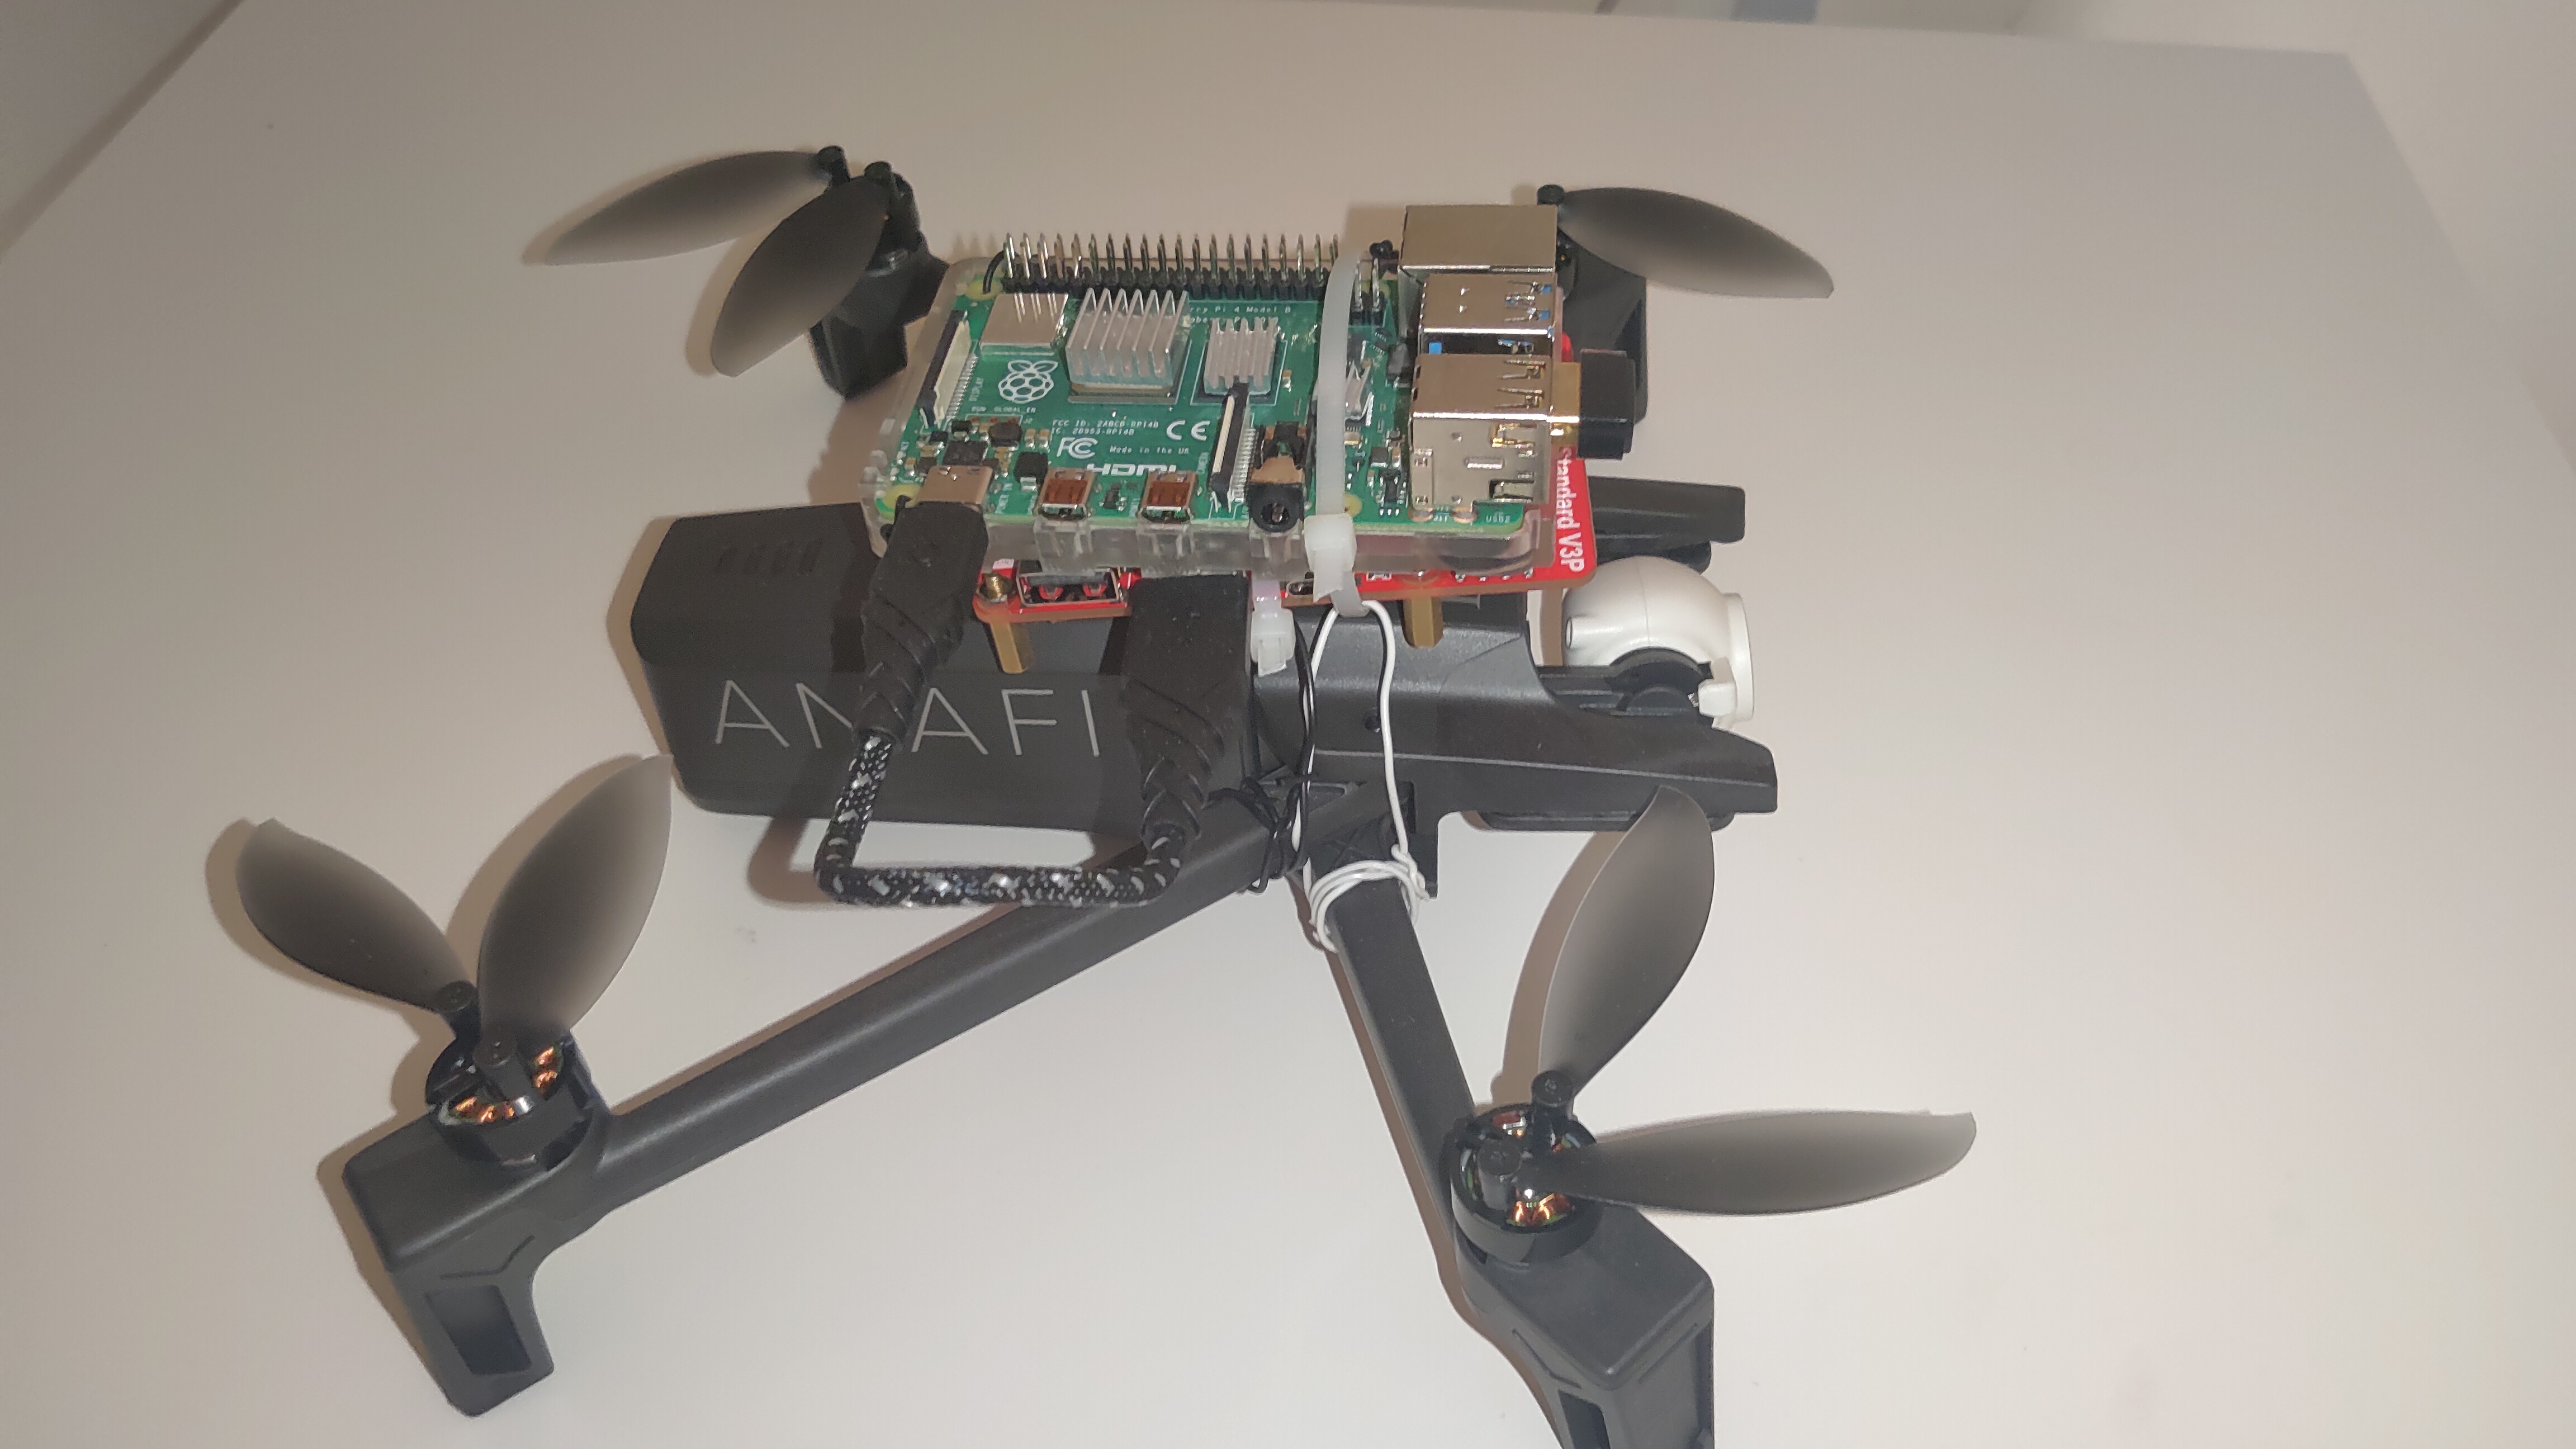
\includegraphics[width=0.5\textwidth]{full-hardware.jpg}
	\caption{Full hardware system.}
	\label{fig:full-hardware}
\end{figure}  

\subsection{Reinforcement learning}

\lipsum[1]

\subsection{User interface}

\lipsum[1]

\end{document}
